\chapter{Аналитическая часть}
\section{Описание объектов сцены}

Сцена состоит из следующих объектов:
\begin{itemize}
	\item камера --- объект, которым может управлять пользователь, с которого осуществляется наблюдение за сценой;
	\item точечный источник света --- объект, положение которого совпадает с положением камеры, освещает сцену;
	\item модель --- объект, который может быть отображен на сцене и который может быть отредактирован пользователем.
\end{itemize}

\section{Анализ и выбор формы задания трехмерных моделей}
В компьютерной графике существует три основных способа задания трехмерной модели.
\begin{enumerate}
	\item Каркасная (проволочная) модель --- простейшая форма задания трехмерной модели. В этом случае необходимо хранить только вершины --- точки, привязанные к координатной сетке и ребра --- линии, связывающие вершины.
	
	\item Поверхностная модель --- самый популярный вид трехмерной модели в компьютерной графике. Она состоит из вершин, ребер и полигонов. Однако минусом данного вида является незнание того, на какой стороне располагается текстура.\newpage
%	В свою очередь поверхностные модели подразделяются на модели заданные сплайновым способом --- способ задания модели характеризуется описанием объекта, которое доступно в неявной форме, то есть для получения визуальных характеристик необходимо дополнительно вычислять некоторую функцию, которая зависит от параметра, и заданные полигональной сеткой --- данный способ характеризуется совокупностью вершин, граней и ребер, которые определяют форму многогранного объекта в трехмерной компьютерной графике. Существет несколько видов хранения полигональной сетки: 
%	\begin{itemize}
%		\item список граней --- объект представляется множеством граней и множеством вершин, в каждую грань входят как минимум 3 вершины;
%		\item «крылатое» представление --- каждая точка ребра указывает на две вершины, две грани и четыре ребра, которые её касаются;
%		\item полурёберные сетки --- то же «крылатое» представление, но информация обхода хранится для половины грани;
%		\item таблица углов, хранящая вершины; обход заданной таблицы неявно задаёт полигоны;
%		\item вершинное представление --- хранятся лишь вершины, которые указывают на другие вершины.	
%	\end{itemize}
	\item Объемная (твердотельная) модель --- данная форма отличается от поверхностной тем, что у нас есть информация о том, где расположен материал, это делается с помощью указания направления внутренней нормали. 
\end{enumerate}

Для выполнения задания выбраны поверхностные модели. Полигоны, ребра и вершины будут храниться в хэш-таблицах для уменьшения времени доступа к ним.
%Таким образом для выполнения задания мы будем опираться на поверхностные модели, заданные полигональной сеткой. При этом полигональная сетка будет задаваться динамическим списком граней, и дополнительно будут храниться динамические списоки ребер --- для отрисовки модели без отсечения и точек --- для предотвращения дублирования математических операций при переносе, повороте и маштабировании нескольких объектов, в которые входит один и тот же элемент. Это позволит удобно работать с каждым компонентом по отдельности и вместе.

\section{Анализ методов вывода трехмерных объектов на экран}

Существует три основных алгоритма отображения объемного тела на плоскости.
\begin{enumerate}
	\item Трассировка лучей --- из точки наблюдения на объекты сцены направляются лучи, с помощью которых определяется цвет пикселя на двумерном экране при попадании луча в модель; при этом луч не прекращает своё распространение, а разделяется на три луча-компонента, каждый из которых вносит свой вклад в цвет пикселя на двумерном экране: отражённый, теневой и преломлённый. Благодаря своим особенностям, метод позволяет получить очень фотореалистичные изображения, однако из-за большой ресурсоёмкости процесс визуализации занимает значительное время.
	\item Рэйкастинг --- метод похожий на трассировку лучей, различие состоит в том, что при нахождении первого пересечения с моделью лучи прекращают своё распространение. Возможно использование каких-либо очень простых способов добавления оптических эффектов. Эффект перспективы получается естественным образом в случае, когда бросаемые лучи запускаются под углом, зависящим от положения пикселя на экране и максимального угла обзора камеры.
	\item Растеризация --- метод, состоящий из двух этапов: вершинный шейдер, при котором каждый полигон и грань модели проходят процесс переспективного преобразования, и самого этапа растеризации, где по известным вершинам (в данном случае уже пикселям на экране) необходимо получить все остальные пиксели модели и их атрибуты (цвет, текстура, глубина). 
\end{enumerate}
Будут реализованы два алгоритма: растеризация --- это ускорит отрисовку сцены в режиме реального времени, и рэйкастинг --- данный алгоритм будет так же использован в выборе элемента щелчком мыщи с тем отличием, что будет рассматриваться не весь экран, а только выбранный пиксель.
\begin{center}
	\centering{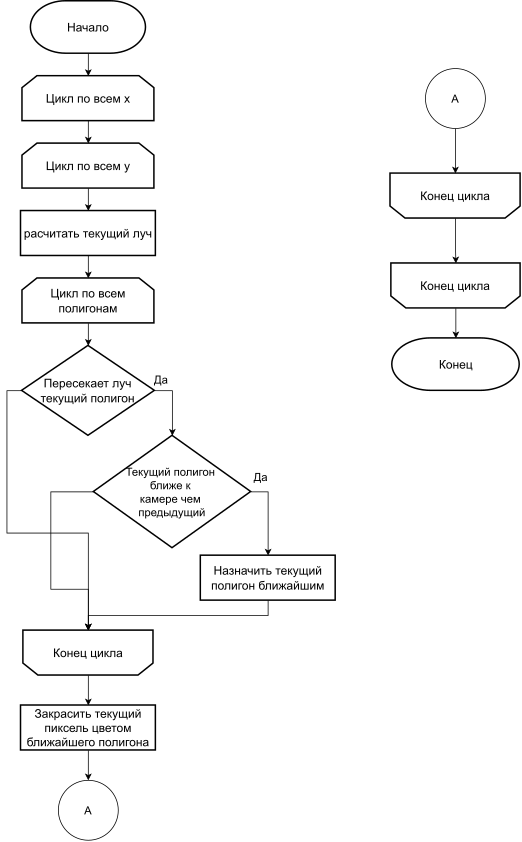
\includegraphics[trim=0 0 0cm 0cm bb=0 0 392 190]{src/raycasting}}
	\captionof{figure}{Процесс работы рэйкастинга}
	\label{img:raycasting}
\end{center}
\section{Описание трёхмерных преобразований}
\subsection{Способ хранения декартовых координат }
Координаты можно хранить в форме вектор-столбца х, у, z. Однако в этом случае неудобно применять преобразования поворота, так как
такой вектор нельзя умножить на соответствующие квадратные матрицы
трансформации размерности четыре на четыре. Целесообразнее использовать вектор-столбцы размерности четыре - [x, y, z, w], где координата $w = 1$.
Преобразования координат выполняются умножением слева преобразуемого вектора-строки на соответствующую матрицу линейного оператора.

\subsection{Матрицы аффинных преобразований декартовых координат}
\begin{enumerate}
	\item Сдвиг точки на $dx$, $dy$, $dz$ по координатным осям:
	\begin{equation}
		\label{eq:T}
		\begin{pmatrix}
			1 & 0 & 0 & 0 \\
			0 & 1 & 0 & 0 \\
			0 & 0 & 1 & 0 \\
			dx & dy & dz & 1 \\
		\end{pmatrix}.
	\end{equation}
	\item Масштабирование относительно начала координат с коэффициентами $sx$, $sy$, $sz$:
	\begin{equation}
	\label{eq:S}
	\begin{pmatrix}
		sx & 0 & 0 & 0 \\
		0 & sy & 0 & 0 \\
		0 & 0 & sz & 0 \\
		0 & 0 & 0 & 1 \\
	\end{pmatrix}.
\end{equation}
	\item Поворот относительно осей $x$, $y$, $z$ соответственно на угол  $\alpha$ :
	\begin{equation}
	\label{eq:X}
		Rx(\alpha) = \begin{pmatrix}
		1 & 0 & 0 & 0 \\
		0 & \cos(\alpha) & \sin(\alpha) & 0 \\
		0 & -\sin(\alpha) & \cos(\alpha) & 0 \\
		0 & 0 & 0 & 1 \\
	\end{pmatrix},
\end{equation}	
\begin{equation}
\label{eq:Y}
Ry(\alpha) = \begin{pmatrix}
	\cos(\alpha) & 0 & -\sin(\alpha) & 0 \\
	0 & 1 & 0 & 0 \\
	\sin(\alpha) & 0 & \cos(\alpha) & 0 \\
	0 & 0 & 0 & 1 \\
\end{pmatrix},
\end{equation}	
\begin{equation}
\label{eq:Z}
Rz(\alpha) = \begin{pmatrix}
\cos(\alpha) & \sin(\alpha) & 0 & 0 \\
	-\sin(\alpha) & \cos(\alpha) & 0 & 0 \\
	0 & 0 & 1 & 0 \\
	0 & 0 & 0 & 1 \\
\end{pmatrix}.
\end{equation}
\end{enumerate}

\subsection{Преобразование трехмерного пространства в двумерное пространство экрана}
Нижеописанные пункты применимы к методу растеризации.

Алгоритм перевода координат из трехмерного пространства к двумерному, следующий \cite{Open}: 
\begin{enumerate}
	\item[1)] перевести объект из мирового пространства в пространство камеры;
	\item[2)] найти все проекции точек из пространства камеры в видимые точки, где координаты точек x, y, z находятся в диапазоне [−w, w], а w находится в диапазоне [0, 1];
	\item[3)] масштабировать все точки, полученные в пункте 2, на картинку необходимого разрешения. 
\end{enumerate}

\subsection{Преобразования трехмерной сцены в пространство камеры}
Для того, чтобы преобразовать сцену в пространство камеры нужно умножить каждую вершину всех полигональных моделей на матрицу
камеры. Сама камера задается набором следующих атрибутов: положение
центра камеры в мировом пространстве, вектора направления взгляда, направления верха камеры.
Матрица камеры представляет собой результат перемножения двух матриц:
\begin{equation}
	\label{eq:Cam}
	 \begin{pmatrix}
		Right_{x} & Right_{y} & Right_{z} & 0 \\
		Up_{x} & Up_{y} & Up_{z}  & 0 \\
		D_{x} & D_{y} & D_{z} & 0 \\
		0 & 0 & 0 & 1 \\
	\end{pmatrix} *  
\begin{pmatrix}
	1 & 0 & 0 & -PX \\
	0 & 1 & 0  & -PY \\
	0 & 0 & 1 & -PZ\ \\
	0 & 0 & 0 & 1 \\
\end{pmatrix},
\end{equation}
где D --- вектор "взгляда" камеры, Up --- вектор, который указывает куда направлен верх камеры, Right --- ортогональный вектор к векторам направления "взгляда" и вектору направления верха камеры.
\subsection{Матрица перспективной проекции}
После перехода в пространство камеры следует умножить каждую
вершину всех полигональных моделей на матрицу проекции (\ref{eq:Proj}). Матрица проекции отображает заданный диапазон усеченной пирамиды \ref{img:proj} в пространство
отсечения, и при этом манипулирует w-компонентой каждой вершины таким образом, что чем дальше от наблюдателя находится вершина, тем
больше становится это w-значение. После преобразования координат в пространство отсечения х, у попадают в диапазон от -w до w, а вершина z от
0 до w (вершины, находящиеся вне этого диапазона, отсекаются). Следующий этап --- спроецировать все координаты на одну плоскость, разделив всё на координату z. После умножения вектора координат на матрицу перспективной проекции, реальная координата z заносится в w-компоненту, так что вместо деления на z делят на w. 
	\begin{equation}
	\label{eq:Proj}
	\begin{pmatrix}
		\dfrac{\cot{\frac{fov}{2}}}{aspect} & 0 & 0 & 0 \\
		0 & \cot{\frac{fov}{2}} & 0 & 0 \\
		0 & 0 & \dfrac{f+n}{f-n} & 1 \\
		0 & 0 & \dfrac{-2fn}{f-n} & 0 \\
	\end{pmatrix}.
\end{equation}
В (\ref{eq:Proj}):
\begin{itemize}
	\item aspect --- отношение ширины изображения к его высоте;
	\item fov --- угол обзора камеры;
	\item f --- координата $z$ дальней от камеры плоскости отсечения пирамиды
	видимости;
	\item n --- координата $z$ ближней к камере плоскости отсечения пирамиды
	видимости
\end{itemize}
\begin{center}
	\centering{\includegraphics[trim=0 0 0cm 0cm bb=0 0 500 340]{src/proj}}
	\captionof{figure}{Усеченная пирамида проекции}
	\label{img:proj}
\end{center}
\subsection{Преобразования трехмерной сцены в пространство области изображения}
Чтобы преобразовать спроецированные координаты в координаты области изображения, нужно инвертировать ось Y и  применить операции преноса и маштабирования к каждой вершине.

\section{Анализ алгоритма удаления невидимых ребер и поверхностей}
\subsection{Z-буфер}
Суть данного алгоритма --- это использование Z-буфера, в котором хранятся информация о координате Z для каждого пикселя.
Первоначально в Z-буфере находятся максимально возможные значения Z. Каждый многоугольник преобразуется в растровую форму.
В процессе подсчета глубины нового пикселя, он сравнивается с тем значением, которое уже лежит в Z-буфере. Если новый пиксель расположен ближе к наблюдателю, чем предыдущий, то онотрисовывается и происходит корректировка Z-буфера. Необходимо отметить, что в данном алгоритме может возникнуть следующая ситуация: если два объекта имеют близкую Z-координату, то они могут перекывать друг друга. Это называется Z-конфликт (рис. \ref{img:zc}). Решаются Z-конфликты сдвигом одного объекта относительно другого на величину, превышающую погрешность Z-буфера.
\begin{center}
	\centering{\includegraphics[trim=0 0 0cm 0cm bb=0 0 330 330]{src/zc}}
	\captionof{figure}{Z-конфликт}
	\label{img:zc}
\end{center}

\section{Алгоритмы растреризации}
\subsection{Интерполяция}
Интерполяция \cite{cg} --- в вычислительной математике нахождение неизвестных промежуточных значений некоторой функции, по имеющемуся дискретному набору её известных значений, определенным способом. Для каждого полигона необходимо провести интерполяцию по двум осям: X и Y. Сначала происходит интерполяция по каждому ребру для нахождения промежуточных значений, затем для каждой сканирующий строки происходит интерполяция по X, что позволяет получить данные о каждой точке внутри полигона. Данный алгоритм позволяет довольно быстро определить цвет, глубину и остальные атрибуты для элемента. 
\subsection{Traversal алгоритм}
Барицентрические координаты --- это координаты, в которых точка
треугольника описывается как линейная комбинация вершин. Чаще всего используют нормализованный вариант
--- т.е. суммарный вес трех вершин равен единице

%\begin{center}
%	\centering{\includegraphics[trim=0 0 0cm 0cm bb=0 0 200 200]{src/bary}}
%	\captionof{figure}{Представление барицентрических координат}
%	\label{img:b}
%\end{center}
Барицентрические координаты равны отношению площадей треугольников, образованных на \ref{img:bs}, к общей площади треугольника:
\begin{equation}
	b_{0} = \frac{\delta_{0}}{\delta},
	b_{1} = \frac{\delta_{1}}{\delta},
		b_{2} = 1 - b_{0} - b_{1}.
\end{equation}

\begin{center}
	\centering{\includegraphics[trim=0 0 0cm 0cm bb=0 0 200 200]{src/bary_s}}
	\captionof{figure}{Площади полигона}
	\label{img:bs}
\end{center}
Значение атрибута в заданной точке треугольника равно линейной комбинации барицентрических координат и значений атрибута в соответствующих вершинах:
\begin{equation}
	T = b_{0}*T_{0} + b_{1}*T_{1} + b_{2}*T_{2}
\end{equation}

Данный алгоритм работает в соответствии с нижележащими пунктами:
\begin{itemize}
	\item определить наименьший прямоугольник, описывающий полигон;
	\item для каждого пикселя выбранного прямоугольника определить барицентрицеские координаты
	\item если значение каждой из них находится в отрезке от 0 до 1, то находим атрибуты рикселя и закрашиваем его.
\end{itemize}

\subsection*{Вывод}
Не смотря на то, что алгоритм интерполяции выполняется быстрее по времени из-за того, что он работает исключительно в пространстве полигона, будут реализованы оба алгоритма по условию задания.

\section{Модель освещения}
В программе будет использована простая модель освещения, суть которой заключается в следующем: вся грань закрашивается одним уровнем интенсивности,который высчитывается по закону Ламберта. 
